\documentclass[a4paper, 12pt]{article}
\usepackage{comment} % enables the use of multi-line comments (\ifx \fi) 
\usepackage{lipsum} %This package just generates Lorem Ipsum filler text. 
\usepackage{fullpage} % changes the margin
\usepackage{indentfirst}
\usepackage{graphicx}
\graphicspath{{./images/}}
\usepackage[colorlinks=true,linkcolor=black,urlcolor=cyan]{hyperref}
\usepackage{fancyvrb}
\newcommand{\myTilde}{$\sim$}
\begin{document}
%Header-Make sure you update this information!!!!
\noindent
\large\textbf{Understanding Git\footnote{\url{https://github.com/progit/progit2/releases/download/2.1.82/progit.pdf}}} \hfill \textbf{Filippo Cesaratto} \\
\normalsize

\section*{What is git?}
Git is a type of \textbf{version control system} (VCS) that makes it easier to track changes to files. For example, when you edit a file, git can help you determine exactly \emph{what} changed, \emph{who} changed it, and why.

It's useful for coordinating work among multiple people on a project, and for tracking progress over time by saving ``checkpoints''. 

\section*{The three states}
Each file in the \emph{working directory} can be in one of these two states: \emph{tracked} or \emph{untracked}. Tracked files are the files that git knows about. In fact these files had to be present in the last \emph{snapshot} git took, and can have one of these three possible states:
\paragraph{Committed/Unmodified} This means that the data is safely stored in your local database.
\paragraph{Modified} This means that you have changed your file, but have not committed it to your database yet. You have to use the command \textbf{add} to \emph{stage} it.
\paragraph{Staged} This means that you have marked a modified file in its current version to go into your next commit snapshot.

\vspace*{5mm}
\begin{figure}[h]
	\centering
	\includegraphics{FilesStates}
\end{figure}

\section*{Basic commands}
Below is a series of basic commands with descriptions of what they each do.

\paragraph{git help $<$command$>$} This opens the browser and displays information about the given \textbf{command}. If a refresher is all that it's needed, just type: \textbf{git $<$command$>$ -h}.

\paragraph{git init}
This starts your own \emph{repository} from scratch in any existing directory on your computer. Git stores information about changes of the local (in the directory $D$ where git is initialized) files in a data structure called a \emph{repository}. This \emph{repository} is stored in a \emph{.git} directory inside the directory $D$ that is called the \emph{working directory}. No file of the directory $D$ is tracked yet.

\paragraph{git clone $<$URL$>$ [$<$directoryName$>$]}
This downloads an existing repository from the internet to your computer and extract the latest \emph{snapshot}. Almost all the files are downloaded so there is the possibility to open a previous snapshot of the downloaded project. By default it will be saved in the same directory where your repository is in, using the same name as the downloading snapshot, but if the optional parameter \textbf{directoryName} is given, then that would be its name.

\paragraph{git status}
This will print some basic information, such as which files have recently been modified. An option to shorten its content is \textbf{git status -s}.

\paragraph{git add $<$fileName$>$}
This adds \textbf{fileName} to the staged files that will be committed once the \textbf{commit} command is called. It's a multipurpose command: tracks new files, stages modified tracked files, and other things. Think as ``it adds precisely this content to the next commit''. There's the possibility of adding all the files in a directory; instead of inserting the file name, just insert the directory name in the \textbf{fileName} field. 

\paragraph{.gitignore}
This is not a command; it's a file in the root directory that git looks at to see if some of the files in that repository have to be shown (as \emph{untracked}) or not when calling the \textbf{status} command. A .gitignore file is a sequence of rules that prevent files to be looked at. An example (the text after the pound symbol is ignored):
\begin{verbatim}
	#ignore all .a files in this directory
	*.a
	#but do track lib.a, even though you're ignoring .a files above
	!lib.a
	#ignore TODO file in this directory
	/TODO
	#ignore all files in the build directory
	build/
	#ignore all the txt files in the subdirectory doc,
	#but not the subdirectory doc/server
	doc/*.txt
	#ignore all pdf files in doc and all its subdirectories
	doc/**/*.pdf	
\end{verbatim}

\paragraph{git diff} This lets you know what lines have been changed to a modified file since its last staging. This means the file was added to the stage files, and then edited. You can see the difference between what is going to be committed (\emph{staged} file) and the file as it is in this moment after the changing (\emph{modified} file). To compare the last commit (\emph{unmodified} file) to the staged changes (\emph{staged} file) the command is \textbf{git diff -{}-staged}. This doesn't look at the modified file that is not staged yet. Be careful: this flag could cause you to include unwanted changes to your files.

\paragraph{git commit} This commits all the \emph{staged} files. This means that those staged files and all the previously committed files (but not staged) will be inserted in a \emph{snapshot} of the project. Adding a \textbf{-v} option will insert a \textbf{git diff -{}-staged} in the message so you can see exactly the changes you're committing. Another option is \textbf{-m} that lets you type the message between quotation marks without opening the text editor. There's an option to skip the \emph{stage} phase for files that are already tracked: \textbf{-a}. This means that \emph{modified} files can directly go to the \emph{committed}/\emph{unmodified} files without them being \emph{staged}, hence without using the \textbf{add} command.

\paragraph{git rm $<$fileName$>$} This removes the file \textbf{fileName} from the tracked list and from the directory. If \textbf{fileName} is a staged file, its removal has to be forced using the \textbf{-f} option. If you're only interested in not keeping track of it anymore, but you wish the file to be not deleted, just add the option \textbf{-{}-cached}. This is particularly useful if you forgot to add something to your \textbf{.gitignore} file. Instead of a file, \textbf{fileName} could be a directory or file patterns; two example could be:
\begin{Verbatim}[commandchars=+\[\]]
   $ git rm log/\*.log
   $ git rm \*+myTilde
\end{Verbatim}
The first removes all the \verb|.log| files inside the directory \verb|log/| (the backslash \verb|\| is needed because git has its own interpreter), whilst the second removes all the files whose names end with a $\sim$.

\paragraph{git mv $<$oldFileName$>$ $<$newFileName$>$} This changes the name of a file. This \textbf{newFileName} will be \emph{staged}, ready to be committed. Git doesn't keep track of file movement, so if this command is not used, \textbf{oldFileName} has to be removed, and then \textbf{newFileName} has to be added. If a file has its name changed in the explorer window, there's the needing of remove and add the same file with different names.

\paragraph{git log} This lists all the commits that were made in reverse chronological order. Lots of options for this command (\textbf{git help log}). One of the more used is the \textbf{-p} option that shows all the changes introduced in each commit (\textbf{git diff} attached to the main log). To show only the last $n$ entries, the option is \textbf{-$n$} (e.g., \textbf{-3} for the last 3 entries). The \textbf{-{}-stat} option shows some stats of the logs (number of changed files and lines). The option \textbf{-S $<$text$>$} only shows logs of changed \textbf{text} for two different \emph{commits}.

\paragraph{git commit -{}-amend} This commit takes your staging files and uses them for the commit. This new commit deletes the previous one and writes its own. This is useful if you forgot some minor changes that you can do and commit without typing in the message something like ``Typo corrected''.

\paragraph{git reset HEAD $<$fileName$>$} This is useful when you've changed two files and both are wrongly added to the staging area, but you don't want to make a single commit for those two changes. This requires to remove the staged status from one of these files (\textbf{fileName}). This unstages the file.

\paragraph{git checkout -{}- $<$fileName$>$} This unmodifies \textbf{fileName} deleting it and reapplying its previous \emph{committed} status. Any changes made to the file are gone for good.

\section*{Remote repository commands}

\paragraph{git remote add $<$nickName$>$ $<$URL$>$}  This adds a new remote git repository. The \textbf{nickName} parameter is used for easily reference that on-line repository. This reference is created once and there is no need to reconnect to the on-line repository.

\paragraph{git remote} This alone shows if there are remote repositories linked to the off-line one. Adding the option \textbf{-v}, it shows the URL of this repository with information about the \emph{push} and \emph{fetch} options (writing and reading respectively).

\paragraph{git fetch $<$nickName$>$} Using the \textbf{nickName} previously given to the on-line repository, this downloads commits, files and refs from a remote repository into your local one. You use this command when you want to see what everybody else has been working on. It doesn't merge the changes into your repository. Fetching is a safe way to review commits before integrating them with your local repository.

\paragraph{git push $<$nickName$>$ $<$branch$>$} This command saves the \textbf{branch} of your local repository (e.g. \textbf{master}) to the \textbf{nickName} on-line one. There is the possibility that this command fails if someone else has made changes that are not \textbf{fetched} yet.

\paragraph{git remote show $<$nickName$>$} This shows the URL and the tracking branch information.

\paragraph{git remote rename $<$nickName$>$ $<$newNickName$>$} This changes the remote-tracking \emph{nick name}.

\paragraph{git remote remove $<$nickName$>$} This lets you remove a \textbf{nickName} from the server. Once you delete the reference to a remote this way, all remote-tracking branches and configuration settings associated with that remote are also deleted. 

\section*{Tagging commands}

\paragraph{git tag} This command lists the tags in alphabetical order. An optional parameter is \textbf{-l $<$tagName$>$} as for example \textbf{-l \texttt{"{}}v1.5*\texttt{"{}}} that lists all the tags that starts with the given \emph{tagName} (v1.5.1, v1.5.2, etc).

\paragraph{git tag -a $<$tagName$>$ -m $<$message$>$} This command creates an \emph{annotated} tag named \textbf{tagName} and attach the \textbf{message} to it. \emph{Annotated} tags are stored as full objects in the repository. They are checksummed; contain the tagger name, email, and date; have a tagging message; and can be signed and verified with GNU Privacy Guard.

















\section*{Branching}

\paragraph{git branch $<$newBranchName$>$}
This creates a local checkpoint technically called a \emph{reference} with the given \textbf{newBranchName}. A branch is an active line of development. The most recent commit on a branch is referred as the tip of that branch.

\paragraph{git checkout $<$existingBranchName$>$}


































\end{document}
